% !TEX program = XeLaTeX
\documentclass{VUMIFPSkursinis}
    \usepackage{algorithmicx}
    \usepackage{algorithm}
    \usepackage{algpseudocode}
    \usepackage{amsfonts}
    \usepackage{amsmath}
    \usepackage{bm}
    \usepackage{caption}
    \usepackage{color}
    \usepackage{enumitem}
    \usepackage{float}
    \usepackage{graphicx}
    \usepackage{listings}
    \usepackage{subfig}
    \usepackage{wrapfig}
    \usepackage{booktabs}
    \usepackage{blindtext}
    \usepackage{colortbl}
    \usepackage{graphicx}
    \usepackage{multirow}
    \usepackage{scrextend}
    \usepackage{longtable}
    \usepackage{enumitem}
    \usepackage{xparse}
    %\usepackage{tabularx}
    \usepackage{ltxtable}
    \usepackage{tabu}
    \usepackage{xcolor}
    % Titulinio aprašas
    \university{Vilniaus universitetas}
    \faculty{Matematikos ir informatikos fakultetas}
    \department{Programų sistemų katedra}
    \papertype{Laboratorinis darbas}
    \title{Skrydžių bilietų paieškos sistema}
    \titleineng{Plane tickets search system}
    \status{2 kurso 4 grupės studentai}
    \author{Vardenis Pavardenis}
    \secondauthor{Vardenis Pavardenis}
    \thirdauthor{Vardenis Pavardenis}
    \fourthauthor{Vardenis Pavardenis}
    \date{Vilnius – \the\year}
    
    % Nustatymai
    % \setmainfont{Palemonas}   % Pakeisti teksto šriftą į Palemonas (turi būti įdiegtas sistemoje)
    \bibliography{bibliografija}
    
    \begin{document}
    \maketitle
      
        \tableofcontents
      
        \sectionnonum{Įvadas}
              Šiame dokumente bus aprašyti sistemos "Skrydžių bilietų paieška" reikalavimai, struktūrinės dalykinės srities modelis ir užduotys. Reikalavimai išskirstyti į funkcinius ir nefunkcinius. Funkciniai reikalavimai nurodo pagrindines sistemos funkcijas, o nefunkciniai - nurodo kaip tas funkcijas sistema turi atlikti. Struktūrinės dalykinės srities modelis yra pateikiamas UML klasių diagramomis kartu su žodynais - sąrašu esybių su jų aprašymais. Paskutiniame skyriuje pateikiamos sistemos užduotys su jų aprašymais.
        \section{Reikalavimai}
            \subsection{Funkciniai reikalavimai}
                \begin{enumerate}[label=\textbf{FR\arabic*}.]
                    \item Sistema turi galėti atlikti skrydžių paiešką pagal paieškos kriterijus.
                    \item Paieškos kriterijai sudaromi iš:
                    \begin{itemize}
                    	\item išvykimo ir atvykimo datų intervalų (nuo/iki),
                    	\item skrydžio kainos intervalo (nuo/iki),
                    	\item išvykimo ir atvykimo vietų.
                    \end{itemize}
                    \item Vartotojui norint įvesti datą, sistema turi pateikti mažą kalendorių arba leisti vartotojui savarankiškai įvesti datą.
                    \item Paieškos formoje nieko neįvedus arba įvedus netinkamai, sistema turi pateikti vartotojui pavyzdį, kaip turėtų būti suvesti duomenys.
                    \item Sistema turi turėti galimybę rūšiuoti ir/arba  filtruoti paieškos rezultatus.
                    \begin{enumerate}[label*=\textbf{\arabic*}.]
                        \item Sistema rūšiuoja skrydžius pagal:
                        \begin{itemize}
                            \item greičiausius,
                            \item pigiausius,
                            \item optimaliausius (žr. \ref{optimal}).
                        \end{itemize}
                        \item Sistema filtruoja skrydžius pagal:
                        \begin{itemize}
                            \item aviakomapanijas,
                            \item persėdimų skaičių.
                        \end{itemize}
                    \end{enumerate}
                    \item Pasirinkus skrydį sistema turi parodyti detalią skrydžio informaciją.
                    \item Sistema turi turėti galimybę vartotojui įsigyti skrydžio(-ų) bilietą, nukreipiant jį į atitinkamą aviakompanijos puslapį.
                    \item Sistema atitinkamame lange vartotojui turi parodyti būsimus skrydžius, į kuriuos jis įsigijo bilietus.
                \end{enumerate}
            \subsection{Nefunkciniai reikalavimai}
                \begin{enumerate}[label=\textbf{NFR\arabic*}.]
                    \item Turi būti palaikoma operacinė sistema su viena iš naršyklių:
                    \begin{itemize}
                        \item Mozilla Firefox (nuo 58 versijos)
                        \item Google Chrome (nuo 64 versijos)
                        \item Microsoft Internet Explorer (nuo 11 versijos)
                        \item Microsoft Edge (nuo 41 versijos)
                        \item Apple Safari (nuo 11 versijos)
                    \end{itemize}
                    \item Turi būti palaikomas HTTPS standartas.
                    \item Programų sistema turi būti susieta su aviakompanijų bilietų pirkimo svetaine.
                    \item Programų sistema turi turėti prieigą prie duomenų bazės, kurioje saugomi tvarkaraščiai, naudotojai, įvykiai ir užrašai.
                    \item Datos įvedamos ir vaizduojamos DD/MM/YYYY formatu.
                    \item Išvykimo data turi būti anksčiau arba sutapti su atvykimo data.
                    \item Skrydžio kainos turi būti teigiamos ir rodomos eurais.
                    \item Mažiausia skrydžio kaina turi būti mažesnė už didžiausią skrydžio kainą.
                    \item Išvykimo ir atvykimo vietos negali sutapti.
                    \item Vieta vaizduojama arba vedama formatu "<miestas> <oro uosto trijų raidžių trumpinys>".
                    \item \label{optimal} Optimalesnis skrydis yra tas kurio kainos ir skrydžio trukmės santykis yra mažesnis.
                    \item Detali skrydžio informacija yra:
                    \begin{itemize}
                    	\item skrydžio išvykimo ir atvykimo datos ir laikai,
                    	\item skrydžio išvykimo ir atvykimo šalys, miestai ir oro uosto trumpiniai.
                    \end{itemize}
                    \item Programų sistemos palaikymui yra būtina bent 426 x 240 (240p 16:9) ekrano rezoliucija ir ekrano dydis turi būti bent 4‘‘.
                    \item Įvykus sistemos sutrikimui, vartotojo darbo funkcionalumas turi būti atkurtas penkių minučių laikotarpyje.
                    \item Didžiausia leistina programų sistemos apkrova yra 5000 vartotojų, prisijungusių vienu metu.
                    \item Paieškos rezultatai pateikiami ne lėčiau kaip per 20 sekundžių.
                    \item Programa turi būti įdiegta ir paleista serveryje, kuris veikia visomis metų dienomis 24 valandas per parą.
                    \item Sisteminės klaidos turi būti išsaugojamos klaidų žurnale, kuris turi būti tikrinamas bent kartą per vieną darbo dieną
                    \item Praplėtus programų sistemos funkcionalumą būtina patikrinti atnaujinimus prieš leidžiant jais naudotis vartotojams
                    \item Programų sistema negali pažeisti Europos Žmogaus teisių ir pagrindinių laisvių apsaugos konvencijos
                \end{enumerate}
      
        \section{Struktūrinis dalykinės srities modelis}
            \subsection{Klasių diagrama}
                \begin{figure}[H]
                    \centering
                    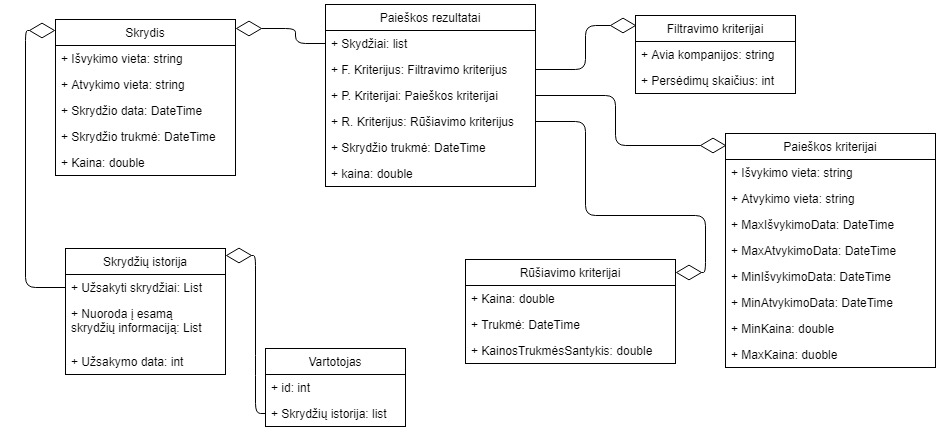
\includegraphics[scale=0.6]{img/class_diagram}
                    \caption{Klasių diagrama}
                    \label{klasių diagrama}
                \end{figure}
                \begin{enumerate}[label=\textbf{E\arabic*}.]
                    \item Paieškos rezultatai - aprašo skrydžių paieškos rezultatus pritaikius paieškos kriterijus.
                    \item Skrydis - detaliai aprašo skrydžio informaciją. Skrydžio informacija susideda iš išvykimo vietos, atvykimo vietos, skrydžio datos, skrydžio trukmės ir kainos.
                    \item Skrydžių istorija - aprašo vartotojo užsakytų, įvykusių bei būsimų skrydžių informaciją.
                    \item Filtravimo kriterijai - aprašo vartotojo nustatytus filtravimo kriterijus. Vartotojas gali pasirinkti norimas avia kompanijas ir pageidaujamų persėdimų skaičių
                    \item Paieškos kriterijai - aprašo vartotojo pasirinktus skrydžio bilietų paieškos kriterijus. Vartotojas gali nustatyti išvykimo vietą, atvikimo vietą, maksimalią ir minimalią išvykimo bei atvykimo datą, maksimalią bei minimalią kainą.
                    \item Vartotojas - asmuo naviguojantis skrydžių paieškos platformoje ir ieškantis reikiamų skrydžių.
                \end{enumerate}
    
            \subsection{Reikalavimų - struktūrinio dalykinės srities modelio atsekamumo matrica}
            \begin{center}
                \begin{tabular}{|c|c|c|c|c|c|c|c|c| }
                \hline
                    & FR1 & FR2 & FR3 & FR4 & FR5 & FR6 & FR7 & FR8 \\ 
                \hline
                 E1 & X   &     &     &     & X   &     & X   & X    \\  
                \hline
                 E2 &     &     &     &     &     & X   & X   & X    \\ 
                \hline
                 E3 &     &     &     &     &     &     &     &      \\ 
                \hline
                 E4 &     &     &     &     & X   &     &     &      \\ 
                \hline
                 E5 & X   & X   & X   & X   & X   &     &     &      \\ 
                \hline
                 E6 & X   &     & X   & X   &     &     & X   & X    \\ 
                \hline 
                \end{tabular}
            \end{center}
      
        \section{Užduotys}
            \subsection{Užduočių aprašymai}
            
                \begin{enumerate}[label=\textbf{U\arabic*}.]

                    \item \textbf{Ieškoti skrydžių}\\
                    Vartotojas įveda išvykimo, atvykimo miestus. Pagal pageidavimą, įveda išvykimo ir atvykimo tinkamų laikų intervalus, kainos intervalą. Tada vartotojas paspaudžia ant mygtuko "Ieškoti" ir yra nukreipiamas į paieškos rezultatų langą, kur jam, lentelės pavidalu rodomi surasti skrydžiai pagal vartojojo įvestus kriterijus.
                    \\\textbf{Alternatyvūs scenarijai:}
                    \begin{itemize}
                        \item Jei vartotojas neįveida atvykimo ir/ar išvykimo miestų, jam paspaudus ant mygtuko "Ieškoti" jis nėra nukreipiamas į rezultatų langą. Išvykimo ar atvykimo miesto įvedimo laukas su neįvesta reikšme (arba abu), paženklinami raudonai.
                    \end{itemize}

                    \item \textbf{Rušiuoti paieškos rezultatus}\\
                    Paieškos rezultatų lange, vartotojas pasirenka vieną iš trijų rūšiavimo būdus atitinkančių mygtukų: "Greičiausias", "Pigiausias" arba "Optimalus". Paspaudus ant vieno iš jų, skrydžių paieškos rezultatai yra surūšiuojami pagal pasirinktą rušiavimo būdą.
                    \\\textbf{Alternatyvūs scenarijai:}
                    \begin{itemize}
                        \item Surušiavus rezultatus tam tikru pasirinktu būdu, vartotojas paspaudžia ant jau pasirinktą rūšiavimo būdą atitinkančio mygtuko. Rezultatai lieka surūšiuoti taip pat kaip ir prieš spaudžiant. 
                    \end{itemize}

                    \item \textbf{Filtruoti paieškos rezultatus}\\
                    Paieškos rezultatų lange, vartotojas pažymi jį dominantį persėdimų skaičių ir skrydžių bendrovę. Vartotojui pažymėjus konkrečią reikšmę ar to, ar ano, paieškos rezultatai yra iš karto atnaujinami, vaizduojant tik tuos skrydžius, kurie tenkina filtrų reikšmes.
                    \\\textbf{Alternatyvūs scenarijai:}
                    \begin{itemize}
                        \item Vartotojui pakartotinai paspaudus ant jau prieš tai pažymėta filtro reikšmės, rezultatai iš karto atsinaujina, o konkretus pažymėtas filtras nuimamas. Kai visi filtrai yra nuimti, rezultatai atsivaizduoja netaikant jiems jokio filtravimo.
                    \end{itemize}

                    \item \textbf{Pereiti į bilieto pardavėjo svetainę}\\
                    Vartotojas atlieka skrydžių paiešką. Spaudžia ant pasirinkto skrydžio iš sąrašo ir yra nukeliamas į bilieto pardavėjo puslapį.

                    \item \textbf{Peržiūrėti būsimų skrydžių sąrašą}\\
                    Vartotojas spaudžia ant mygtuko "Būsimi skrydžiai". Atidaromas skrydžių, į kuriuos vartotojas yra įsigijęs bilietus sąrašas.
                    \begin{figure}[H]	
                        \centering
                        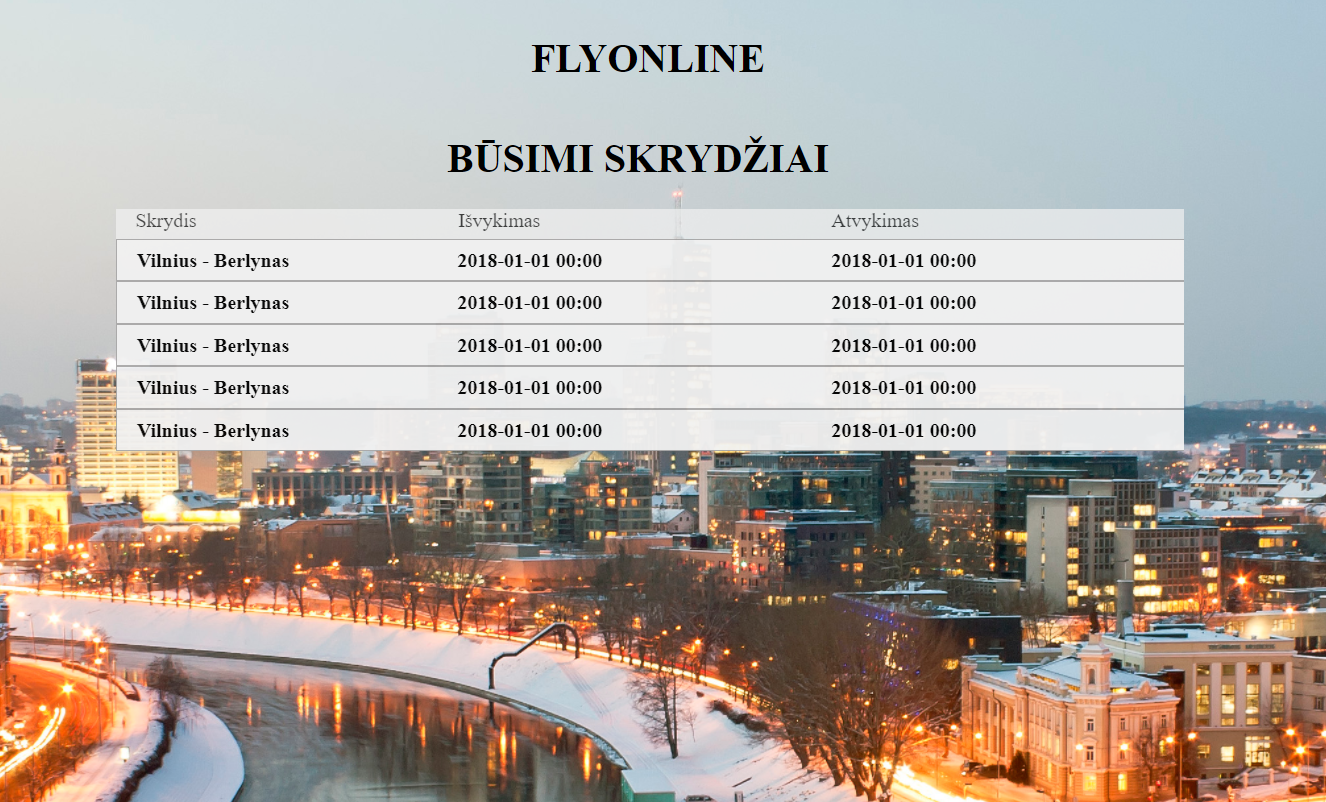
\includegraphics[scale=0.4]{img/history}	
                        \caption{Būsimų skrydžių sąrašas}	
                        \label{Būsimų skrydžių sąrašas}	
                    \end{figure}
                    \textbf{Alternatyvūs scenarijai:}
                    \begin{itemize}
                        \item Jei būsimų skrydžių sąrašas yra tuščias, sąrašo vietoje vartotojui parodoma žinutė "Sąrašas yra tuščias.";
                    \end{itemize}

                    \item \textbf{Peržiūrėti detalią skrydžio informaciją}\\
                    Vartotojas atidaro būsimų skrydžių sąraša. Spaudžia ant pasirinkto skrydžio iš sąrašo ir yra atidaromas dialogas su išsamia skrydžio informacija.
                    \begin{figure}[H]	
                        \centering
                        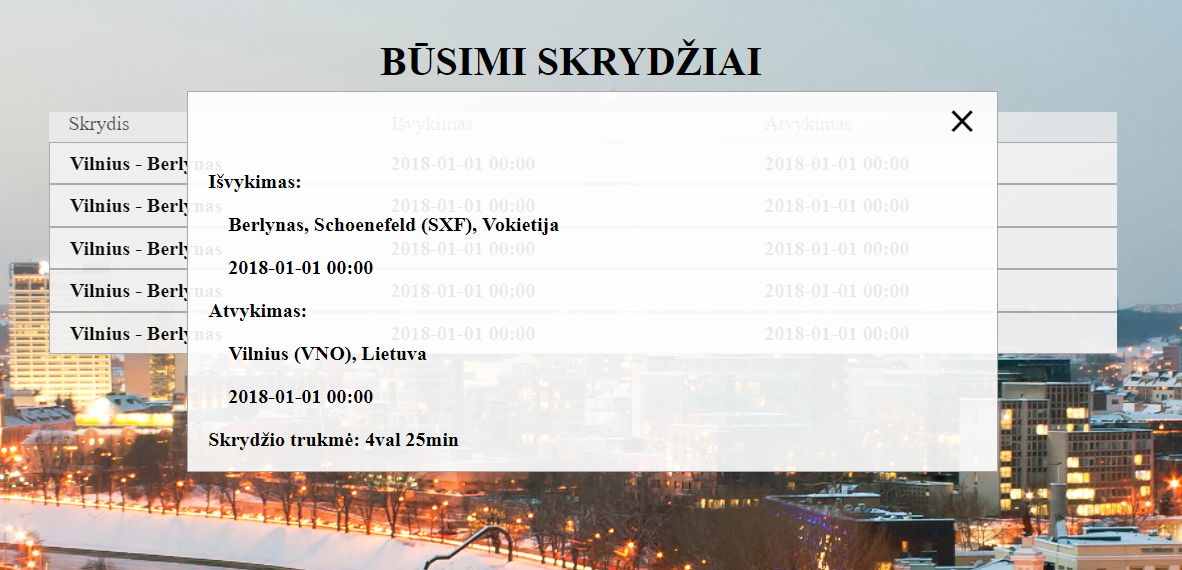
\includegraphics[scale=0.4]{img/details}	
                        \caption{Skrydžio informacija}	
                        \label{Skrydžio informacija}	
                    \end{figure}
                    
                \end{enumerate}
      
            \subsection{Reikalavimų - užduočių atsekamumo matrica}
            \begin{center}
                \begin{tabular}{|c|c|c|c|c|c|c|c|c| }
                \hline
                    & FR1 & FR2 & FR3 & FR4 & FR5 & FR6 & FR7 & FR8 \\ 
                \hline
                 U1 & X   & X   & X   & X   &     &     &     &      \\  
                \hline
                 U2 &     &     &     &     & X   &     &     &      \\ 
                \hline
                 U3 &     &     &     &     & X   &     &     &      \\ 
                \hline
                 U4 &     &     &     &     &     &     & X   &      \\ 
                \hline
                 U5 &     &     &     &     &     &     &     & X    \\ 
                \hline
                 U6 &     &     &     &     &     & X   &     & X    \\ 
                \hline 
                \end{tabular}
            \end{center}

        \sectionnonum{Išvados}
			Sistemos dokumentacija papildyta naujais reikalavimais, o kai kurie buvę reikalavimai patikslinti. Viskas daryta atsižvelgiant į užsakovų norus ir logika. Sistema yra paruošta kūrimo pradžiai.
        \sectionnonum{Šaltiniai}
    
        \appendix  % Priedai
        % Prieduose gali būti pateikiama pagalbinė, ypač darbo autoriaus savarankiškai
        % parengta, medžiaga. Savarankiški priedai gali būti pateikiami ir
        % Priedai taip pat numeruojami ir vadinami. Darbo tekstas
        % su priedais susiejamas nuorodomis.
      
    \end{document}
      